\chapter{MULTI-PORT RAM}
\label{chapter:scratchpad}
Our multi-port RAM was created to allow mutliple processing elements to use a shared memory. It is a component in the larger design for a sparse matrix vector multiplier. Specifically it allows the decoder to access more memory space without going off chip. The component allows each PE to access a table that is 16 times larger than if it was stored inside each PE. Multi-port RAMs have been designed before, but none seemed to have the desired performance.
\section{Design}
The scratchpad is made up of several smaller components. The obviously being the need for block memory.
\begin{figure*}
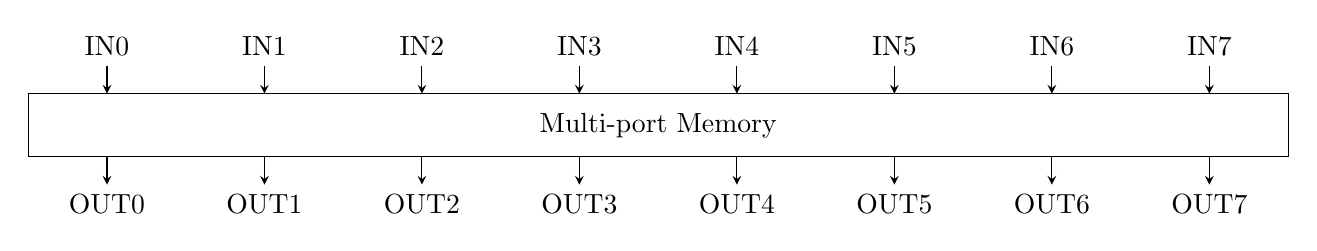
\begin{tikzpicture}[xscale=2]

\foreach \x in {0,1,...,7}{
    \node at (\x,0)(in){IN\x};
    \node at (\x,-2)(out){OUT\x};
    \path[draw,>=stealth,->] (in) -> (\x,-.6);
    \path[draw,>=stealth,->] (\x,-1.4) -> (out);
}
\draw (-.5,-1.4) rectangle (7.5,-.6);
\node at (3.5,-1) {Multi-port Memory};
\end{tikzpicture}
\caption{This model is impossible to achieve in real life. There is no way to scale the design by only $O(n)$. However there will be no problems simulating this design. It also gives us a clear goal of what we want to get as close to as possible.}
\label{fig:gold}
\end{figure*}
\begin{sidewaysfigure}
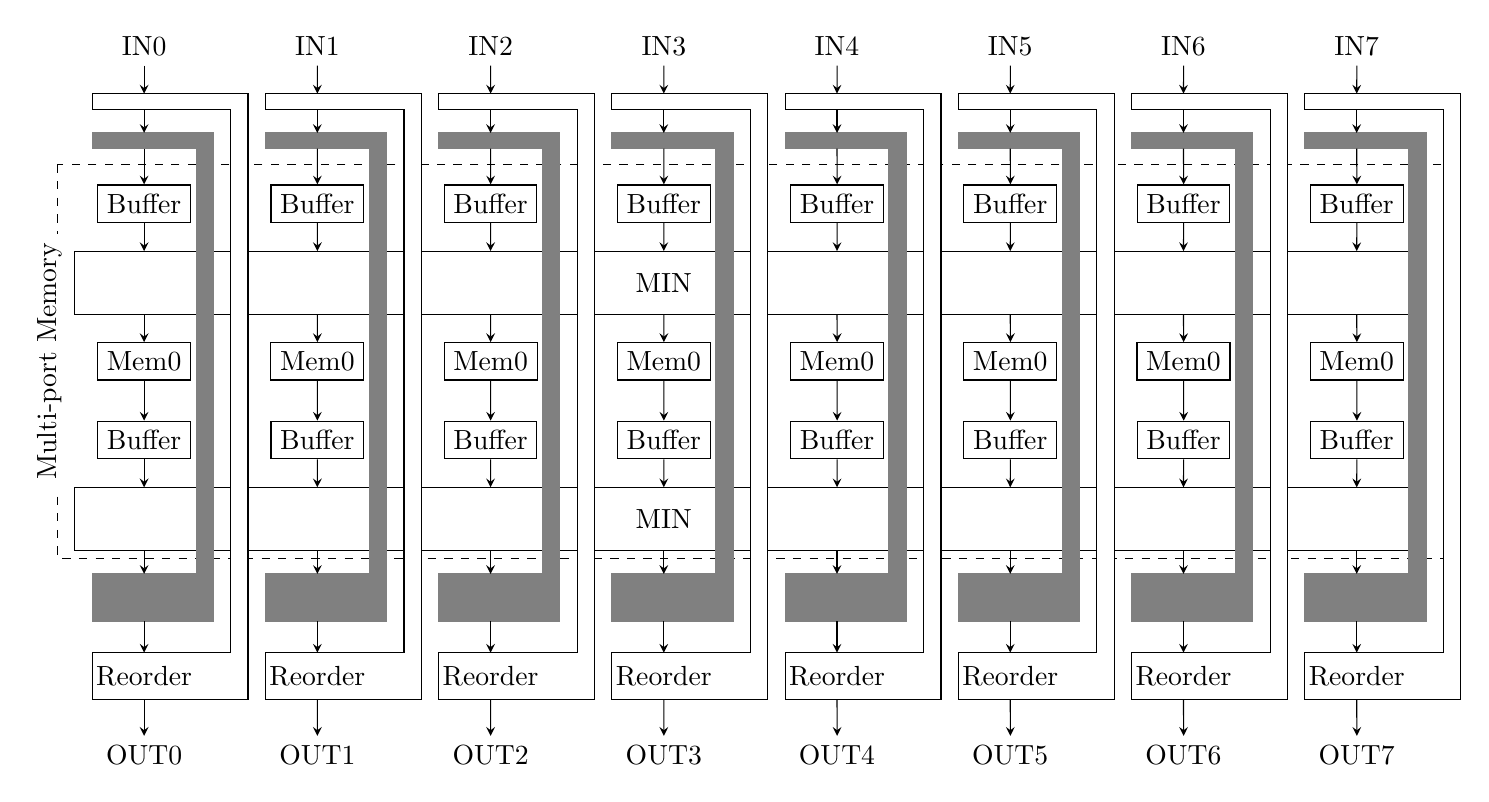
\begin{tikzpicture}[xscale=2.2]
\draw (-.4,-2.6) rectangle (7.4,-3.4);
\draw (-.4,-5.6) rectangle (7.4,-6.4);
\draw[dashed] (-.5,-1.5) rectangle (7.5,-6.5);
\foreach \x in {0,1,...,7}{
    \node at (\x,0)(in){IN\x};
    \node at (\x,-9)(out){OUT\x};
    \draw[xshift=\x cm,fill=white](-.3,-.6) -- (-.3,-.8) -- (.5,-.8) -- (.5,-7.7) -- (-.3,-7.7) -- (-.3,-8.3) -- (.6,-8.3) -- (.6, -.6) -- cycle;
    \node at (\x, -8){Reorder};
    \draw[xshift=\x cm,fill=white,gray](-.3,-1.1) -- (-.3,-1.3) -- (.3,-1.3) -- (.3,-6.7) -- (-.3,-6.7) -- (-.3,-7.3) -- (.4,-7.3) -- (.4, -1.1) -- cycle;
    \node at (\x, -7)[gray]{Cache};
    \node[draw] at (\x,-2)(inBuf){Buffer};
    \node[draw] at (\x,-4)(mem){Mem0};
    \node[draw] at (\x,-5)(outBuf){Buffer};
    \path[draw,>=stealth,->] (in) -- (\x,-.6);
    \path[draw,>=stealth,->] (\x,-.8) -- (\x,-1.1);
    \path[draw,>=stealth,->] (\x,-1.3) -- (inBuf);
    \path[draw,>=stealth,->] (inBuf) -- (\x,-2.6);
    \path[draw,>=stealth,->] (\x,-3.4) -- (mem);
    \path[draw,>=stealth,->] (mem) -- (outBuf);
    \path[draw,>=stealth,->] (outBuf) -- (\x,-5.6);
    \path[draw,>=stealth,->] (\x,-6.4) -- (\x,-6.7);
    \path[draw,>=stealth,->] (\x,-7.3) -- (\x,-7.7);
    \path[draw,>=stealth,->] (\x,-8.3) -- (out);
}
\node at (3,-3){MIN};
\node at (3,-6){MIN};
\node[xshift=-3,rotate=90,fill=white] at (-.5,-4){Multi-port Memory};
\end{tikzpicture}
\caption{High-level view of f-scratch}
\end{sidewaysfigure}
\subsection{Memory Block}
BlockRAMs are the efficient large memory blocks. 16 are used because of the larger space and the need to have 16 ports so that 16 memory operations can occur 
in parallel. We have multiple options to decide how the address space works. The simpliest would be to assign the first 16th addresses to memory0, the next 16th to memory1 etc. However, in our use case the lower addresses are used more, so this would lead to uneven access and therefore bottlenecks. So we use an interleaving memory address space.
\subsection{Cross Bar}
\subsection{Reorder Queue}
\subsection{Tiny Cache}
\section{Conclusion}
